% Manual de instalación y uso de la app del gemelo digital en Windows
% Compilar desde esta carpeta:  pdflatex manual_windows.tex (dos veces)
\documentclass[a4paper,11pt]{article}
% Estilo común de los manuales del gemelo digital (se incluye con \input)
\usepackage{geometry}
\geometry{letterpaper, margin=2.2cm}
\usepackage[spanish, es-nodecimaldot, mexico]{babel}
\usepackage[utf8]{inputenc}
\usepackage[T1]{fontenc}
\usepackage{lmodern}
\usepackage{amsmath,amssymb}
\usepackage[table]{xcolor}
\definecolor{naranja}{RGB}{194,98,12}
\definecolor{rojo}{RGB}{192,57,43}
\definecolor{verde}{RGB}{30,120,70}
\definecolor{azulw}{RGB}{0,103,184}
\definecolor{azulg}{RGB}{70,90,120}
\definecolor{gris}{RGB}{242,242,242}
\definecolor{grisos}{RGB}{90,90,90}
\usepackage{booktabs,longtable,array,tabularx}
\usepackage{graphicx}
\usepackage{float}
\usepackage{caption}
\captionsetup{font=small, labelfont=bf}
\usepackage{tikz}
\usetikzlibrary{positioning,arrows.meta,fit,calc,shapes.geometric,decorations.pathreplacing,backgrounds}
\usepackage{enumitem}
\setlist{itemsep=2pt}
\usepackage{listings}
\lstset{basicstyle=\ttfamily\small, frame=single, backgroundcolor=\color{gris}, breaklines=true,
  columns=fullflexible, keepspaces=true, extendedchars=true, upquote=true,
  literate={á}{{\'a}}1 {é}{{\'e}}1 {í}{{\'i}}1 {ó}{{\'o}}1 {ú}{{\'u}}1 {ñ}{{\~n}}1 {Á}{{\'A}}1 {É}{{\'E}}1
           {Í}{{\'I}}1 {Ó}{{\'O}}1 {Ú}{{\'U}}1 {Ñ}{{\~N}}1 {ü}{{\"u}}1 {¿}{{?`}}1 {¡}{{!`}}1 {…}{{...}}3
           {θ}{{$\theta$}}1 {·}{{$\cdot$}}1 {«}{{\guillemotleft}}1 {»}{{\guillemotright}}1 {°}{{$^\circ$}}1}
\usepackage{hyperref}
\hypersetup{colorlinks=true, linkcolor=naranja, urlcolor=naranja}
\usepackage{fancyhdr}
\pagestyle{fancy}
\fancyhf{}
\cfoot{\small \thepage}
\newcommand{\codigo}[1]{\texttt{#1}}
\newcommand{\archivo}[1]{\textbf{\texttt{#1}}}
\newcommand{\aviso}[1]{\par\smallskip\noindent\colorbox{rojo!10}{\parbox{\dimexpr\linewidth-2\fboxsep}{\textbf{\color{rojo}Atención.} #1}}\par\smallskip}
\newcommand{\nota}[1]{\par\smallskip\noindent\colorbox{gris}{\parbox{\dimexpr\linewidth-2\fboxsep}{#1}}\par\smallskip}
\tikzset{
  marca/.style={circle, fill=naranja, text=white, font=\bfseries\footnotesize, inner sep=1.4pt, minimum size=4.6mm, draw=white, line width=0.8pt},
  caja/.style={draw, rounded corners=2pt, fill=gris, align=center, font=\small, minimum height=10mm, inner sep=4pt},
  cajab/.style={caja, fill=white},
  cajan/.style={caja, fill=naranja!14, draw=naranja!70!black},
  paso/.style={draw, rounded corners=2pt, fill=white, align=left, font=\small, text width=3.4cm, minimum height=15mm, inner sep=5pt},
  num/.style={circle, fill=naranja, text=white, font=\bfseries\small, inner sep=1.5pt, minimum size=6mm},
  flecha/.style={-{Stealth[length=2.2mm]}, thick},
  dflecha/.style={{Stealth[length=2.2mm]}-{Stealth[length=2.2mm]}, thick},
  etiq/.style={font=\scriptsize, align=center},
}
\DeclareRobustCommand{\num}[1]{\tikz[baseline=-0.7ex]\node[marca]{#1};}
% \captura{ancho}{archivo}{marcas en coordenadas 0-1 desde la esquina inferior izquierda}
\newcommand{\captura}[3]{%
  \begin{tikzpicture}
  \node[anchor=south west, inner sep=0, draw=black!25] (img) {\includegraphics[width=#1]{#2}};
  \begin{scope}[x={(img.south east)}, y={(img.north west)}]
  #3
  \end{scope}
  \end{tikzpicture}}
% ventana dibujada (consolas y diálogos): \ventana{ancho}{alto}{título}{contenido}
\newcommand{\ventana}[4]{%
\begin{tikzpicture}
\node[draw=black!50, fill=white, minimum width=#1, minimum height=#2, anchor=north west, inner sep=0] (v) at (0,0) {};
\fill[black!8] (v.north west) rectangle ($(v.north east)+(0,-6mm)$);
\node[anchor=west, font=\scriptsize] at ($(v.north west)+(2mm,-3mm)$) {#3};
\node[anchor=east, font=\scriptsize] at ($(v.north east)+(-2mm,-3mm)$) {--\quad$\square$\quad$\times$};
\node[anchor=north west, inner sep=3mm, text width=#1-6mm, font=\scriptsize\ttfamily, align=left] at ($(v.north west)+(0,-6mm)$) {#4};
\end{tikzpicture}}

\lhead{\small Gemelo digital del brazo XK-JS1-1}
\rhead{\small Manual para Windows}
\newcommand{\abrirapp}{doble clic en \archivo{Gemelo digital.bat} o en el acceso directo del escritorio}

\title{\textbf{Gemelo digital del brazo XK-JS1-1}\\[4pt]\large Manual de instalación y uso en Windows}
\author{ETN-902 / ETN-1034 / ETN-1000 · UMSA · II-2026}
\date{10 de noviembre de 2026}

\begin{document}
\maketitle
\thispagestyle{fancy}

La app del gemelo digital muestra el brazo XK-JS1-1 en 3D, lo sigue en vivo y permite mandarlo desde la PC del laboratorio o desde celulares de la misma red. Es \textbf{una sola app} con un menú de inicio que ofrece tres modos: \emph{Simulación}, \emph{Operación local} y \emph{Operación por red local}. La misma carpeta funciona en Windows y en Linux; este manual cubre \textbf{Windows 10 y 11}.

\tableofcontents
\newpage

% =====================================================================
\section{Resumen}
\begin{figure}[H]
\centering
\begin{tikzpicture}[node distance=4mm]
\node[paso] (p1) {copiar la carpeta\\\codigo{gemelo\_brazo\_}\\\codigo{app}};
\node[paso, right=of p1] (p2) {instalar\\Python 3\\(gratuito)};
\node[paso, right=of p2] (p3) {conectar el cable\\y comprobar su\\puerto COM};
\node[paso, right=of p3] (p4) {doble clic en\\\archivo{Gemelo}\\\archivo{digital.bat}};
\foreach \i in {1,...,4} \node[num] at (p\i.north west) {\i};
\draw[flecha] (p1) -- (p2); \draw[flecha] (p2) -- (p3); \draw[flecha] (p3) -- (p4);
\end{tikzpicture}
\caption{Pasos de la instalación en Windows.}
\end{figure}
No hay que instalar nada más que Python: la app usa solo su biblioteca estándar. La ventana del gemelo se abre con Microsoft Edge, que ya viene con Windows.

% =====================================================================
\section{Qué hay en la carpeta}
\begin{center}\small
\begin{tabularx}{\linewidth}{>{\raggedright}p{5.6cm} >{\raggedright\arraybackslash}X}
\toprule
\textbf{Archivo} & \textbf{Para qué}\\
\midrule
\archivo{Gemelo digital.bat} & Abre la app (menú de modos).\\
\archivo{Probar conexion PLC.bat} & Prueba la conexión con el PLC, \textbf{solo lectura}.\\
\archivo{Crear acceso directo.bat} & Pone el acceso \emph{Gemelo digital del brazo} en el escritorio.\\
\codigo{gemelo\_brazo.py}, \codigo{brazo.py}, \codigo{ppi.py}, \codigo{serie.py}, \dots & La app.\\
\codigo{ui\textbackslash}, \codigo{menu.html} & La interfaz (página del gemelo y menú).\\
\codigo{*.sh} & Lanzadores de Linux (no se usan en Windows).\\
\bottomrule
\end{tabularx}
\end{center}
Al usarla, la app crea: \codigo{usuarios.json}, \codigo{tls\_certificado.pem} y \codigo{tls\_clave.pem} (acceso por red), \codigo{calibracion.json}, \codigo{registro\_gemelo.log} y \codigo{perfil\_ventana\textbackslash} (datos de la ventana de Edge). Son propios de esa PC: no los comparta.

% =====================================================================
\section{Requisitos}
\begin{itemize}
\item \textbf{Windows 10 u 11} (64 bits).
\item \textbf{Python 3.8 o superior}, gratuito desde \url{https://www.python.org/downloads/}.
\item \textbf{Microsoft Edge} (incluido en Windows) o Google Chrome, para la ventana del gemelo.
\item El \textbf{cable USB-PPI} del laboratorio (chip CH340) o un convertidor USB--RS485 (sección \ref{sec:rs485}).
\item Para el acceso por red: la PC y los celulares en la misma red Wi-Fi o router.
\end{itemize}

% =====================================================================
\section{Paso 1: copiar la carpeta}
Copie la carpeta \codigo{gemelo\_brazo\_app} (o descomprima \codigo{gemelo\_brazo\_app.zip}) en un lugar fijo, por ejemplo \codigo{C:\textbackslash GemeloBrazo\textbackslash}.
\nota{Conviene una carpeta \textbf{fuera de OneDrive}: la app guarda ahí sus usuarios, su certificado y su registro. Si Windows muestra \emph{«Windows protegió su PC»} al abrir un \codigo{.bat} copiado de otro equipo, pulse \emph{Más información} $\rightarrow$ \emph{Ejecutar de todas formas}; o, antes de descomprimir, clic derecho sobre el \codigo{.zip} $\rightarrow$ \emph{Propiedades} $\rightarrow$ \emph{Desbloquear}.}

% =====================================================================
\section{Paso 2: instalar Python}
\begin{enumerate}
\item Descargue el instalador desde \url{https://www.python.org/downloads/} (\emph{Download Python 3.x}).
\item Ábralo. En la primera pantalla \textbf{marque la casilla \emph{Add python.exe to PATH}} y pulse \emph{Install Now}.
\end{enumerate}
\begin{figure}[H]
\centering
\begin{tikzpicture}
\node[draw=black!50, fill=white, minimum width=11cm, minimum height=5.6cm, anchor=north west] (v) at (0,0) {};
\fill[black!8] (v.north west) rectangle ($(v.north east)+(0,-6mm)$);
\node[anchor=west, font=\scriptsize] at ($(v.north west)+(2mm,-3mm)$) {Python 3.x (64-bit) Setup};
\node[anchor=north west, font=\large\bfseries] at ($(v.north west)+(4mm,-9mm)$) {Install Python 3.x (64-bit)};
\node[anchor=north west, draw=azulw, thick, fill=azulw!6, text width=7cm, font=\small, inner sep=3mm] at ($(v.north west)+(4mm,-19mm)$) {$\rightarrow$ \textbf{Install Now}};
\node[anchor=north west, font=\small] at ($(v.north west)+(4mm,-32mm)$) {$\rightarrow$ Customize installation};
\node[anchor=north west, font=\small] at ($(v.north west)+(4mm,-40mm)$) {$\boxtimes$\; Use admin privileges when installing py.exe};
\node[anchor=north west, font=\small, draw=rojo, very thick, inner sep=1.5mm] (c) at ($(v.north west)+(3mm,-47mm)$) {$\boxtimes$\; \textbf{Add python.exe to PATH}};
\node[anchor=west, font=\small\bfseries, text=rojo] at ($(c.east)+(4mm,0)$) {$\leftarrow$ marcar};
\end{tikzpicture}
\caption{Primera pantalla del instalador de Python (esquema).}
\end{figure}
\begin{enumerate}[resume]
\item Compruébelo: menú Inicio, \codigo{cmd}, y en el \emph{Símbolo del sistema}:
\begin{lstlisting}
py --version
\end{lstlisting}
Debe responder \codigo{Python 3.x.y}. Si \codigo{py} no se reconoce, ejecute otra vez el instalador, elija \emph{Modify} y marque \emph{py launcher}.
\end{enumerate}
\nota{\textbf{Prueba sin brazo.} Con Python instalado ya puede abrir \archivo{Gemelo digital.bat} y elegir \emph{Simulación} en el menú.}

% =====================================================================
\section{Paso 3: el cable y su puerto COM}
En Windows el cable aparece como un \textbf{puerto COM} (por ejemplo \codigo{COM3}).
\begin{enumerate}
\item Enchufe el cable USB-PPI a la PC y el otro extremo al \textbf{puerto 0} del PLC.
\item Clic derecho en el botón Inicio $\rightarrow$ \emph{Administrador de dispositivos} $\rightarrow$ \emph{Puertos (COM y LPT)}:
\end{enumerate}
\begin{figure}[H]
\centering
\ventana{10cm}{4.2cm}{Administrador de dispositivos}{%
> Monitores\\
> Mouse y otros dispositivos señaladores\\
v Puertos (COM y LPT)\\
\hspace*{5mm}\colorbox{naranja!20}{USB-SERIAL CH340 (COM3)}\\
> Procesadores}
\caption{El cable en el Administrador de dispositivos (el número de COM puede ser otro).}
\end{figure}
\begin{itemize}
\item Si aparece con un \textbf{triángulo amarillo} o como \emph{Dispositivo desconocido}, falta el driver. Normalmente Windows Update lo instala solo. Si no, descargue el driver \textbf{CH341SER} desde la página del fabricante del chip (WCH, \url{https://www.wch-ic.com}).
\item No hace falta anotar el número: la app busca sola en todos los puertos COM, los USB primero.
\item Pruebe la conexión con \archivo{Probar conexion PLC.bat} (solo lee el PLC): debe decir \emph{PLC encontrado}, el programa cargado y mostrar las entradas y salidas.
\end{itemize}
\aviso{Un puerto COM solo lo puede usar un programa a la vez. Si en esta PC está instalado STEP 7-Micro/WIN, ciérrelo antes de abrir la app, y cierre la app antes de cargar un programa con Micro/WIN. En Windows no hace falta la máquina virtual.}

% =====================================================================
\section{Paso 4: abrir la app}
\begin{itemize}
\item Doble clic en \archivo{Gemelo digital.bat}. Para tener el acceso en el escritorio, ejecute una vez \archivo{Crear acceso directo.bat}.
\item Se abren una \textbf{consola} con los mensajes de la app y la \textbf{ventana del gemelo} (Edge en modo aplicación) con el menú de inicio (sección \ref{sec:menu}).
\item Para cerrar la app, cierre la ventana del gemelo o pulse \codigo{Ctrl+C} en la consola.
\end{itemize}
\nota{Si la ventana del gemelo no se abre, edite \archivo{Gemelo digital.bat} (clic derecho $\rightarrow$ \emph{Editar}) y agregue \codigo{-{}-navegador} al final de la línea \codigo{\%PY\% gemelo\_brazo.py \%*}: la app se abrirá en el navegador predeterminado, en \url{http://localhost:8050/}.}

\subsection*{Permitir la app en el firewall (operación por red)}
La primera vez que se elige \emph{Operación por red local}, Windows pregunta si Python puede usar la red:
\begin{figure}[H]
\centering
\begin{tikzpicture}
\node[draw=black!50, fill=white, minimum width=10.5cm, minimum height=4.6cm, anchor=north west] (v) at (0,0) {};
\fill[black!8] (v.north west) rectangle ($(v.north east)+(0,-6mm)$);
\node[anchor=west, font=\scriptsize] at ($(v.north west)+(2mm,-3mm)$) {Alerta de seguridad de Windows};
\node[anchor=north west, font=\small, text width=9.5cm] at ($(v.north west)+(4mm,-9mm)$) {Firewall de Windows Defender bloqueó algunas características de \textbf{Python} en todas las redes públicas y privadas.};
\node[anchor=north west, font=\small] at ($(v.north west)+(4mm,-22mm)$) {$\boxtimes$\; \textbf{Redes privadas}, como las domésticas o del trabajo};
\node[anchor=north west, font=\small] at ($(v.north west)+(4mm,-29mm)$) {$\square$\; Redes públicas};
\node[anchor=south east, draw=azulw, thick, fill=azulw!8, font=\small] at ($(v.south east)+(-30mm,3mm)$) {Permitir acceso};
\node[anchor=south east, draw=black!40, font=\small] at ($(v.south east)+(-3mm,3mm)$) {Cancelar};
\end{tikzpicture}
\caption{Aviso del firewall (esquema): marque \emph{Redes privadas} y pulse \emph{Permitir acceso}.}
\end{figure}
\begin{itemize}
\item Si se canceló por error, quien administra la PC puede permitirlo en un \emph{Símbolo del sistema} abierto \emph{como administrador}:
\begin{lstlisting}
netsh advfirewall firewall add rule name="Gemelo brazo" dir=in action=allow protocol=TCP localport=8443 profile=private
\end{lstlisting}
\item \textbf{La red debe ser «privada»}: \emph{Configuración $\rightarrow$ Red e Internet $\rightarrow$ Wi-Fi (o Ethernet) $\rightarrow$} la red $\rightarrow$ \emph{Tipo de perfil de red: Privada}. En una red «pública» Windows bloquea las conexiones entrantes.
\end{itemize}

\subsection*{Opciones de la línea de comandos}
No hacen falta para el uso normal. Se agregan al final de la línea \codigo{\%PY\% gemelo\_brazo.py \%*} del \codigo{.bat}: \codigo{-{}-modo local} (entra directo a un modo: \codigo{simulacion}, \codigo{local} o \codigo{red}), \codigo{-{}-puerto COM4} (fija el puerto), \codigo{-{}-navegador}, \codigo{-{}-sin-ventana}, \codigo{-{}-puerto-red 9443}.

% =====================================================================
% Uso de la app: común a los manuales de Linux y de Windows (se incluye con \input)
% Antes de incluirlo, el manual define \abrirapp (cómo se abre la app en ese sistema).

% =====================================================================
\section{Seguridad}
\begin{itemize}
\item Mientras alguien tenga el mando del brazo real (en la PC o en un celular), una persona debe estar junto a la \textbf{seta de emergencia} del tablero. El paro de la página no la reemplaza.
\item El \textbf{selector del panel (I0.5)} decide quién manda: en \emph{manual} solo el panel; en \emph{automático} la PC o un operador remoto.
\item Con el brazo real, el mando desde la página está \textbf{deshabilitado} al empezar: hay que marcar una casilla y confirmar. Un solo operador tiene el mando a la vez.
\item Si la app, la página o el cable fallan, el PLC se detiene solo (watchdog de 2~s).
\item Antes de mover el brazo real, hacer siempre el \textbf{homing}.
\item Cada ingreso, cada orden aceptada y cada orden rechazada quedan en \codigo{registro\_gemelo.log}, con hora y usuario.
\end{itemize}

% =====================================================================
\section{El menú de inicio}\label{sec:menu}

Al abrir la app (\abrirapp) aparecen dos ventanas: una \textbf{consola} con los mensajes de la app y la \textbf{ventana del gemelo}, que empieza en el menú:

\begin{figure}[H]
\centering
\captura{\linewidth}{img/menu_inicio.jpg}{
  \node[marca] at (0.05,0.711) {1};
  \node[marca] at (0.05,0.533) {2};
  \node[marca] at (0.05,0.356) {3};
  \node[marca] at (0.05,0.272) {4};
  \node[marca] at (0.59,0.848) {5};
  \node[marca] at (0.59,0.565) {6};
  \node[marca] at (0.05,0.159) {7};
  \node[marca] at (0.905,0.959) {8};
}
\caption{Menú de inicio, con la simulación activa (la tarjeta del modo activo aparece resaltada y su botón dice \emph{Volver al gemelo}).}
\end{figure}
\begin{enumerate}[label=\num{\arabic*}, leftmargin=9mm]
\item \textbf{Simulación}: el brazo se mueve en pantalla con un PLC simulado dentro de la app. No necesita brazo ni cable.
\item \textbf{Operación local}: el gemelo sigue al brazo real y se lo puede mandar desde esta PC. Nadie más puede conectarse. La línea de abajo dice si se detecta el cable.
\item \textbf{Operación por red local}: como la operación local, y además celulares y otras PC de la misma red entran con usuario y contraseña.
\item \textbf{Sin brazo}: con esta casilla, la operación por red usa el PLC simulado; sirve para probar el acceso remoto sin la planta.
\item \textbf{Estado}: modo actual, conexión con el PLC, programa reconocido, quién tiene el mando y puertos serie detectados.
\item \textbf{Usuarios del acceso por red}: crear, cambiar el rol, cambiar la contraseña o quitar usuarios (sección \ref{sec:usuarios}).
\item \textbf{Ir al gemelo}: vuelve a la ventana del gemelo en el modo activo (aparece cuando ya hay un modo elegido).
\item Modo activo (al abrir la app por primera vez dice \emph{Sin modo}).
\end{enumerate}

\begin{center}\small
\begin{tabularx}{\linewidth}{>{\raggedright}p{3.2cm} >{\raggedright}X >{\raggedright}X >{\raggedright\arraybackslash}p{3.3cm}}
\toprule
\textbf{Modo} & \textbf{Para qué} & \textbf{Necesita} & \textbf{Quién se conecta}\\
\midrule
Simulación & aprender, practicar, preparar secuencias & nada & solo esta PC\\
Operación local & ver y mandar el brazo real desde la PC del laboratorio & cable USB-PPI, PLC en RUN & solo esta PC\\
Operación por red local & lo mismo, más supervisión y mando desde celulares & cable, al menos un usuario, misma red & esta PC y usuarios de la red\\
\bottomrule
\end{tabularx}
\end{center}

\textbf{Cambiar de modo.} En la barra superior del gemelo, el botón \textbf{«Menú»} (que muestra el modo activo) vuelve a este menú. Elegir otro modo cambia la conexión sin cerrar la app: al pasar de la simulación al brazo real se conecta con el PLC; al salir de la operación por red se cierra el acceso de los celulares. Al cambiar de modo se suelta el mando de los usuarios remotos.

\begin{figure}[H]
\centering
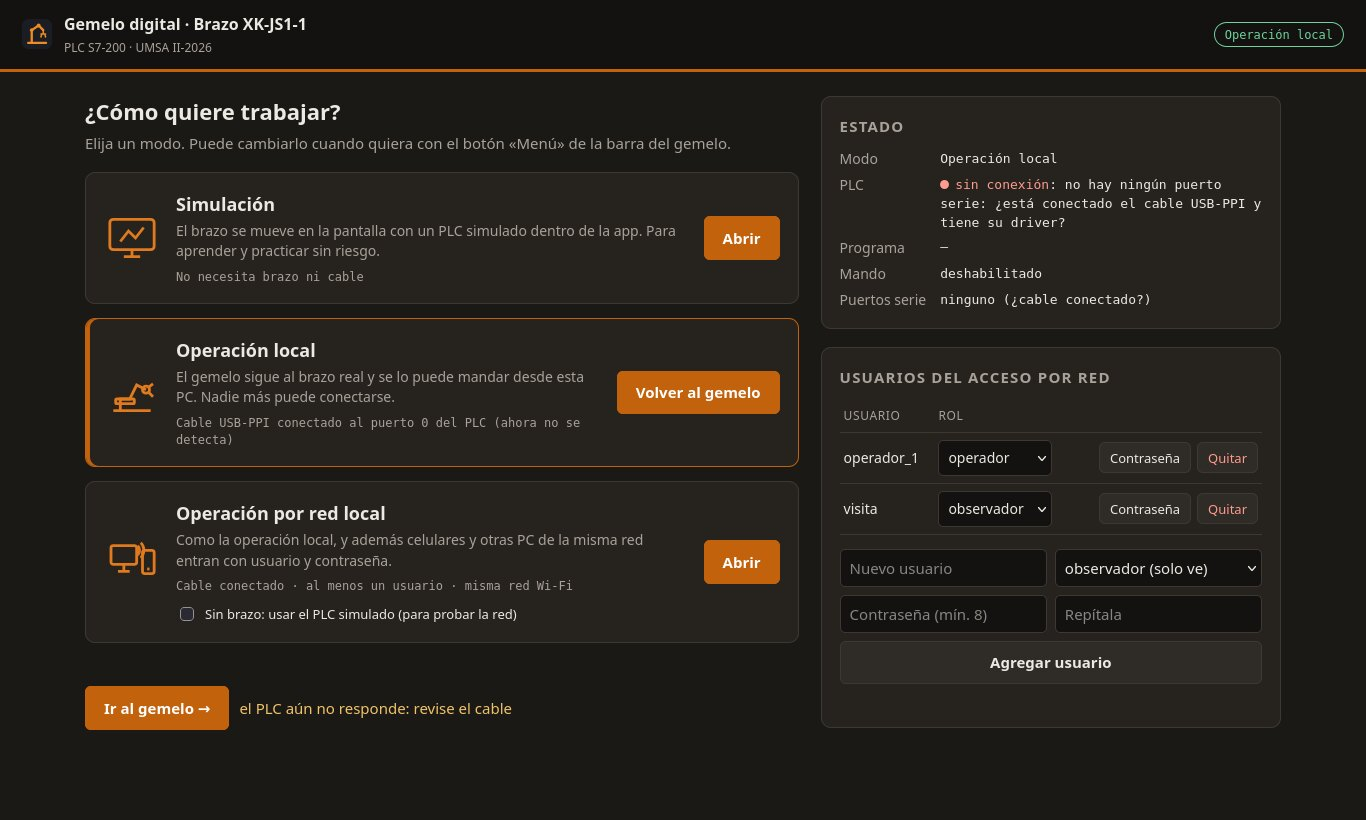
\includegraphics[width=0.92\linewidth]{img/menu_local_sin_cable.jpg}
\caption{Operación local elegida sin el cable conectado: el panel \emph{Estado} explica el motivo. La app sigue buscando el cable cada 2~s y se conecta sola al enchufarlo.}
\end{figure}

% =====================================================================
\section{La ventana del gemelo}\label{sec:gemelo}

La ventana es la misma en los tres modos. Las capturas están hechas en el modo simulación.

\begin{figure}[H]
\centering
\captura{\linewidth}{img/local_articular.jpg}{
  \node[marca] at (0.656,0.925) {1};
  \node[marca] at (0.86,0.925) {2};
  \node[marca] at (0.03,0.86) {3};
  \node[marca] at (0.61,0.855) {4};
  \node[marca] at (0.61,0.77) {5};
  \node[marca] at (0.61,0.505) {6};
  \node[marca] at (0.61,0.42) {7};
  \node[marca] at (0.012,0.094) {8};
  \node[marca] at (0.40,0.094) {9};
  \node[marca] at (0.012,0.048) {10};
}
\caption{Ventana del gemelo, pestaña \emph{Articular}.}
\end{figure}

\begin{enumerate}[label=\num{\arabic*}, leftmargin=9mm]
\item \textbf{Menú}: vuelve al menú de inicio; muestra el modo activo (solo en la PC del laboratorio).
\item \textbf{Estado de la conexión}: PLC conectado, programa reconocido (\emph{gemelo}) y quién tiene el mando.
\item \textbf{Visor 3D}: el brazo en la pose que informa el PLC. Se gira arrastrando con el ratón y se acerca con la rueda.
\item \textbf{Pestañas}: \emph{Articular}, \emph{Cartesiano}, \emph{Secuencias} y \emph{Conexión}.
\item \textbf{Ejes}: $\theta$ de la base, carro X y carro Y. Escriba el valor o suelte el deslizador donde quiera: el brazo va hasta ahí.
\item \textbf{Cerrar garra}, \textbf{Homing} y \textbf{Detener}.
\item \textbf{Velocidad de la simulación} y la casilla que imita el tren de pulsos compartido de X e Y (solo afecta a la simulación de la página).
\item \textbf{Vistas}: isométrica, frontal, lateral y superior.
\item \textbf{Espacio de trabajo} dibuja la zona alcanzable; \textbf{Trayectoria} deja la estela de la garra.
\item \textbf{Indicadores}: conexión, posición estimada, base sin calibrar, selector en manual, falta de homing, errores del PLC.
\end{enumerate}

\begin{figure}[H]
\centering
\captura{\linewidth}{img/local_conexion.jpg}{
  \node[marca] at (0.61,0.70) {1};
  \node[marca] at (0.61,0.58) {2};
  \node[marca] at (0.61,0.49) {3};
  \node[marca] at (0.61,0.43) {4};
  \node[marca] at (0.61,0.335) {5};
  \node[marca] at (0.61,0.245) {6};
}
\caption{Pestaña \emph{Conexión}.}
\end{figure}
\begin{enumerate}[label=\num{\arabic*}, leftmargin=9mm]
\item \textbf{Modo}: \emph{Brazo real (app del gemelo)} sigue a la app; \emph{Simulación} mueve solo el dibujo, sin la app.
\item \textbf{Leer estado}: vuelve a consultar la app.
\item \textbf{PLC y programa} reconocidos.
\item \textbf{Habilitar el mando}: con el brazo real hay que marcarla y confirmar para poder moverlo. En el modo simulación viene marcada.
\item \textbf{Pulsos}: velocidad de los motores, de 500 a 5000~Hz (a 4000~Hz los carros van a 20~mm/s). El programa no tiene rampas: conviene no pasar de 4000~Hz.
\item \textbf{Calibrar la base}: se escribe el ángulo medido con un transportador y la app calcula los pulsos por grado.
\end{enumerate}

\begin{figure}[H]
\centering
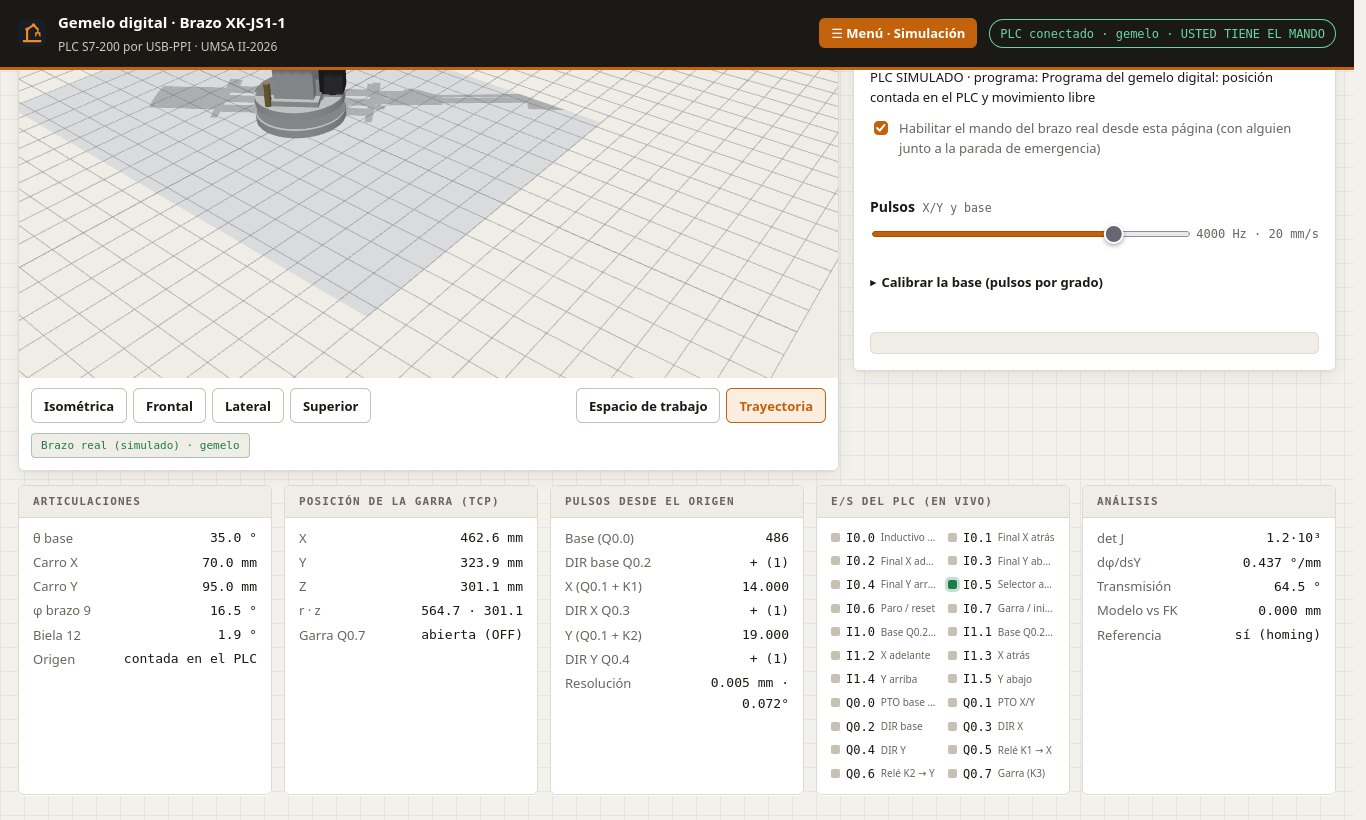
\includegraphics[width=\linewidth, trim=0 0 0 440, clip]{img/local_conexion_abajo.jpg}
\caption{Telemetría, debajo del visor: articulaciones, posición de la garra, pulsos desde el origen, entradas y salidas reales del PLC y análisis (jacobiano, transmisión, referencia).}
\end{figure}

\begin{figure}[H]
\centering
\captura{\linewidth}{img/local_cartesiano.jpg}{
  \node[marca] at (0.61,0.80) {1};
  \node[marca] at (0.61,0.66) {2};
  \node[marca] at (0.61,0.545) {3};
  \node[marca] at (0.61,0.47) {4};
}
\caption{Pestaña \emph{Cartesiano}, con un punto fuera del alcance.}
\end{figure}
\begin{enumerate}[label=\num{\arabic*}, leftmargin=9mm]
\item Origen en el eje de giro sobre la mesa; X apunta al sensor inductivo ($\theta = 0$) y Z hacia arriba.
\item \textbf{X, Y, Z} de la garra en mm.
\item \textbf{Mover} calcula la cinemática inversa y manda las posiciones de los ejes. \textbf{Usar posición actual} copia la posición de la garra en los campos.
\item Si el punto no se alcanza, la página propone el \textbf{punto alcanzable más cercano}; \emph{Usar ese punto} lo copia en los campos.
\end{enumerate}
\nota{\textbf{Por qué muchos puntos salen inalcanzables.} Los carros se mueven en diagonal y la garra solo alcanza una franja estrecha. Justo después del homing el brazo está en una esquina de esa franja: subir o bajar en vertical pide que el carro X retroceda por debajo de cero. Lo práctico es partir de \emph{Usar posición actual} y cambiar los valores de a poco.}

\begin{figure}[H]
\centering
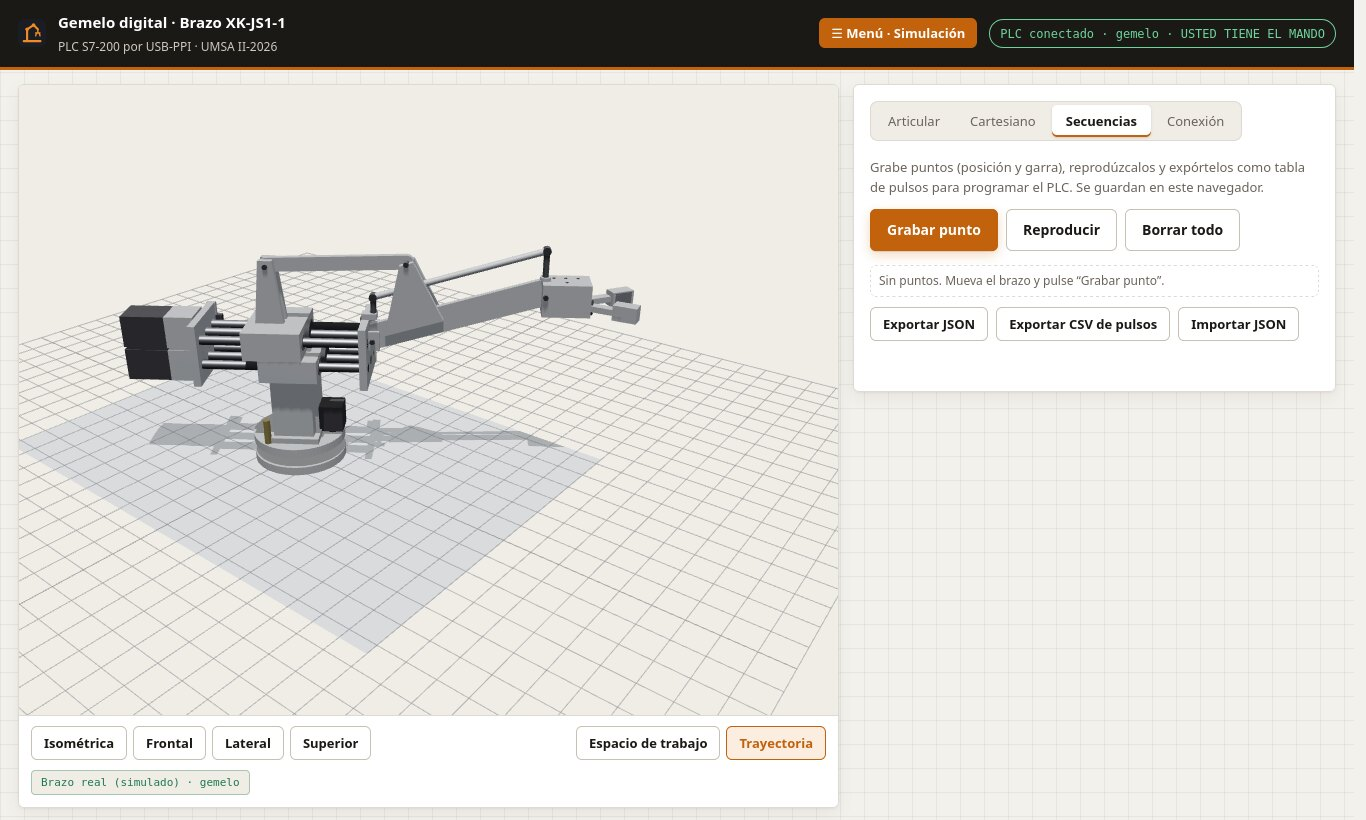
\includegraphics[width=0.9\linewidth]{img/local_secuencias.jpg}
\caption{Pestaña \emph{Secuencias}: \emph{Grabar punto} guarda la posición y la garra; \emph{Reproducir} los recorre esperando que el PLC termine cada uno; se exportan como JSON o como tabla CSV de pulsos.}
\end{figure}

\subsection{Primer uso con el brazo real}
\begin{enumerate}
\item En el menú, \textbf{Operación local} (o por red). Espere a que el estado diga \emph{PLC conectado}.
\item Selector del panel en \emph{automático}.
\item Pestaña \emph{Conexión}: marque \emph{Habilitar el mando} y confirme.
\item Pestaña \emph{Articular}: \textbf{Homing} (Y abajo, X atrás, abre la garra y gira la base al inductivo). Al terminar desaparece \emph{Sin referencia}.
\item Movimientos cortos primero (X 10~mm, Y 10~mm, $\theta$ 5°), comparando con una regla.
\end{enumerate}
Con el programa anterior del PLC (perfil \emph{cargado}) la página es sobre todo un monitor: la posición se estima y solo están las órdenes \emph{Iniciar}, \emph{Detener}, \emph{Paro de emergencia} y \emph{Rearmar}.

% =====================================================================
\section{Usuarios}\label{sec:usuarios}

La operación por red exige usuarios. Se administran en el menú de inicio, en el panel \emph{Usuarios del acceso por red}; solo se puede hacer desde la PC del laboratorio.

\begin{figure}[H]
\centering
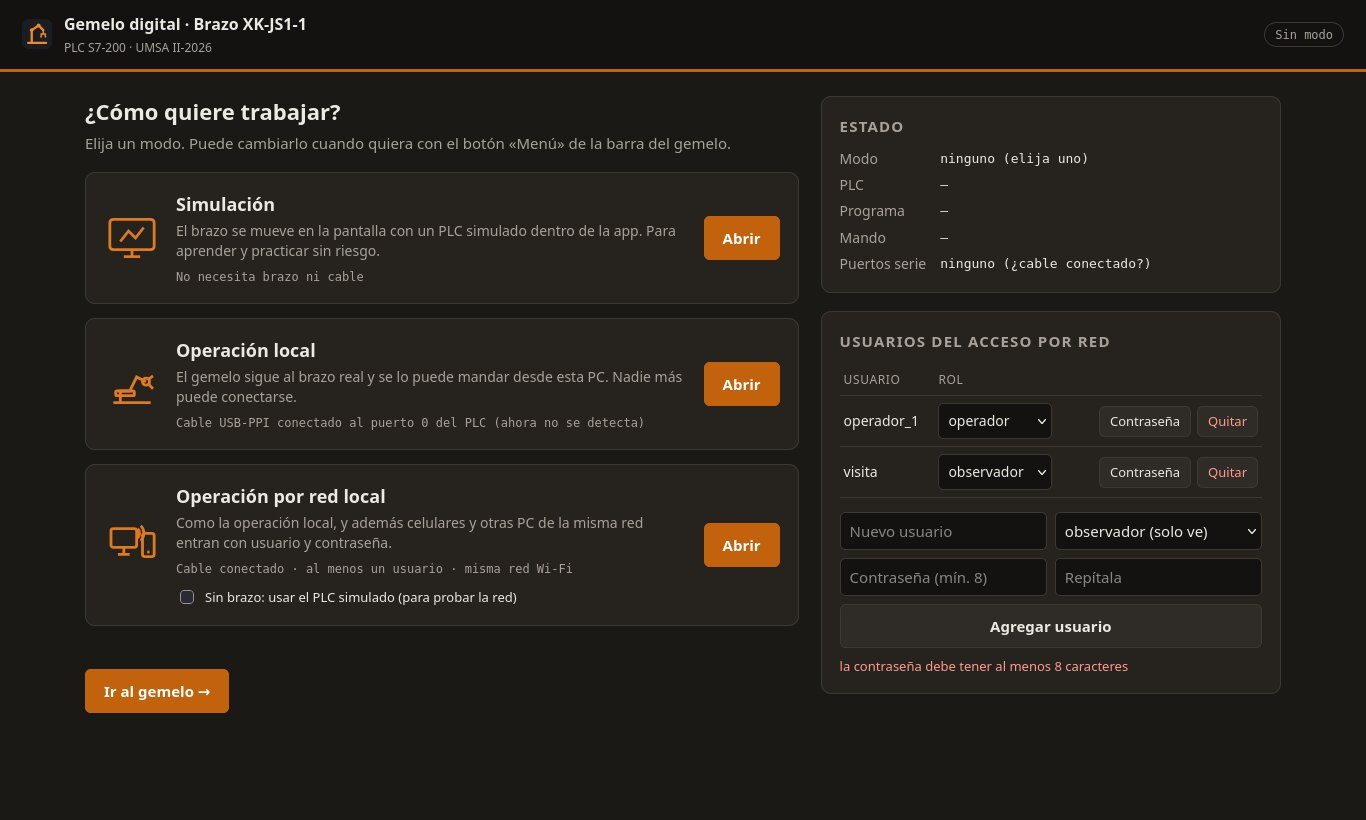
\includegraphics[width=0.92\linewidth]{img/menu_usuarios.jpg}
\caption{Panel de usuarios con dos usuarios creados. Al intentar crear uno con una contraseña corta, el menú lo rechaza y explica el motivo.}
\end{figure}

\begin{itemize}
\item \textbf{Agregar}: nombre (letras, números, punto, guion o guion bajo), rol y contraseña dos veces (al menos 8 caracteres).
\item \textbf{Rol}: el menú desplegable de cada fila lo cambia al momento.
\item \textbf{Contraseña}: pide la nueva dos veces. No hay forma de leer la anterior.
\item \textbf{Quitar}: pide confirmación; si ese usuario tenía el mando, lo pierde.
\end{itemize}

\begin{center}\small
\begin{tabularx}{\linewidth}{>{\raggedright}p{2.6cm} >{\raggedright\arraybackslash}X}
\toprule
\textbf{Rol} & \textbf{Qué puede hacer}\\
\midrule
observador & Ver el brazo en vivo: modelo 3D, posición, entradas y salidas. No puede mover, tomar el mando ni dar paro.\\
operador & Todo lo anterior, más tomar el mando y mover el brazo. Un solo operador tiene el mando a la vez; los demás ven quién lo tiene y pueden dar paro. El mando se suelta al desmarcar la casilla, al pulsar \emph{Salir} o tras 8~h sin uso.\\
\bottomrule
\end{tabularx}
\end{center}
Las contraseñas se guardan cifradas (PBKDF2) en \codigo{usuarios.json}, junto a la app. El nombre distingue mayúsculas. Tras 5 contraseñas erradas desde un equipo, ese equipo espera 60~s. Los usuarios también se pueden administrar desde una terminal con \codigo{usuarios.py} (\codigo{agregar}, \codigo{clave}, \codigo{rol}, \codigo{quitar}, \codigo{listar}).

% =====================================================================
\section{Operación por red local}\label{sec:red}

\begin{enumerate}
\item En el menú, \textbf{Operación por red local} (con la casilla \emph{Sin brazo} para probar con el PLC simulado). La primera vez la app crea el certificado del laboratorio; tarda unos segundos.
\item El panel \emph{Estado} muestra la dirección para los celulares, con un botón \emph{Copiar}:
\end{enumerate}

\begin{figure}[H]
\centering
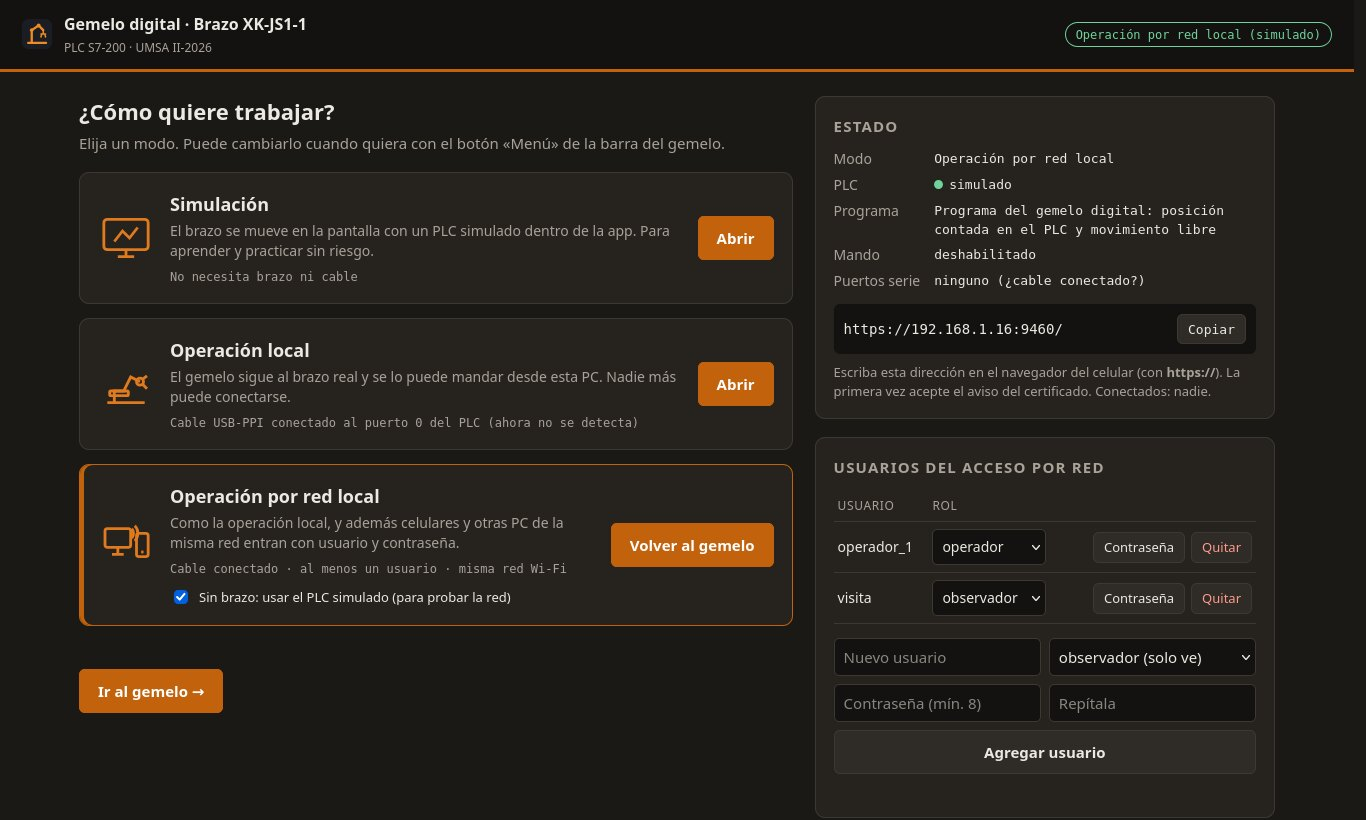
\includegraphics[width=0.92\linewidth]{img/menu_red.jpg}
\caption{Operación por red local activa: la dirección \texttt{https://IP:8443/} y quiénes están conectados.}
\end{figure}

\begin{enumerate}[resume]
\item Conecte el celular \textbf{al mismo Wi-Fi o router} que la PC del laboratorio (con datos móviles no funciona).
\item Escriba la dirección \textbf{con \codigo{https://} y con el puerto \codigo{:8443}}. La primera vez el navegador avisa que la conexión no es privada: el certificado es propio del laboratorio. Pulse \emph{Avanzado $\rightarrow$ Continuar}.
\item Ingrese con su usuario y contraseña.
\end{enumerate}

\begin{figure}[H]
\centering
\begin{minipage}[t]{0.31\linewidth}\centering
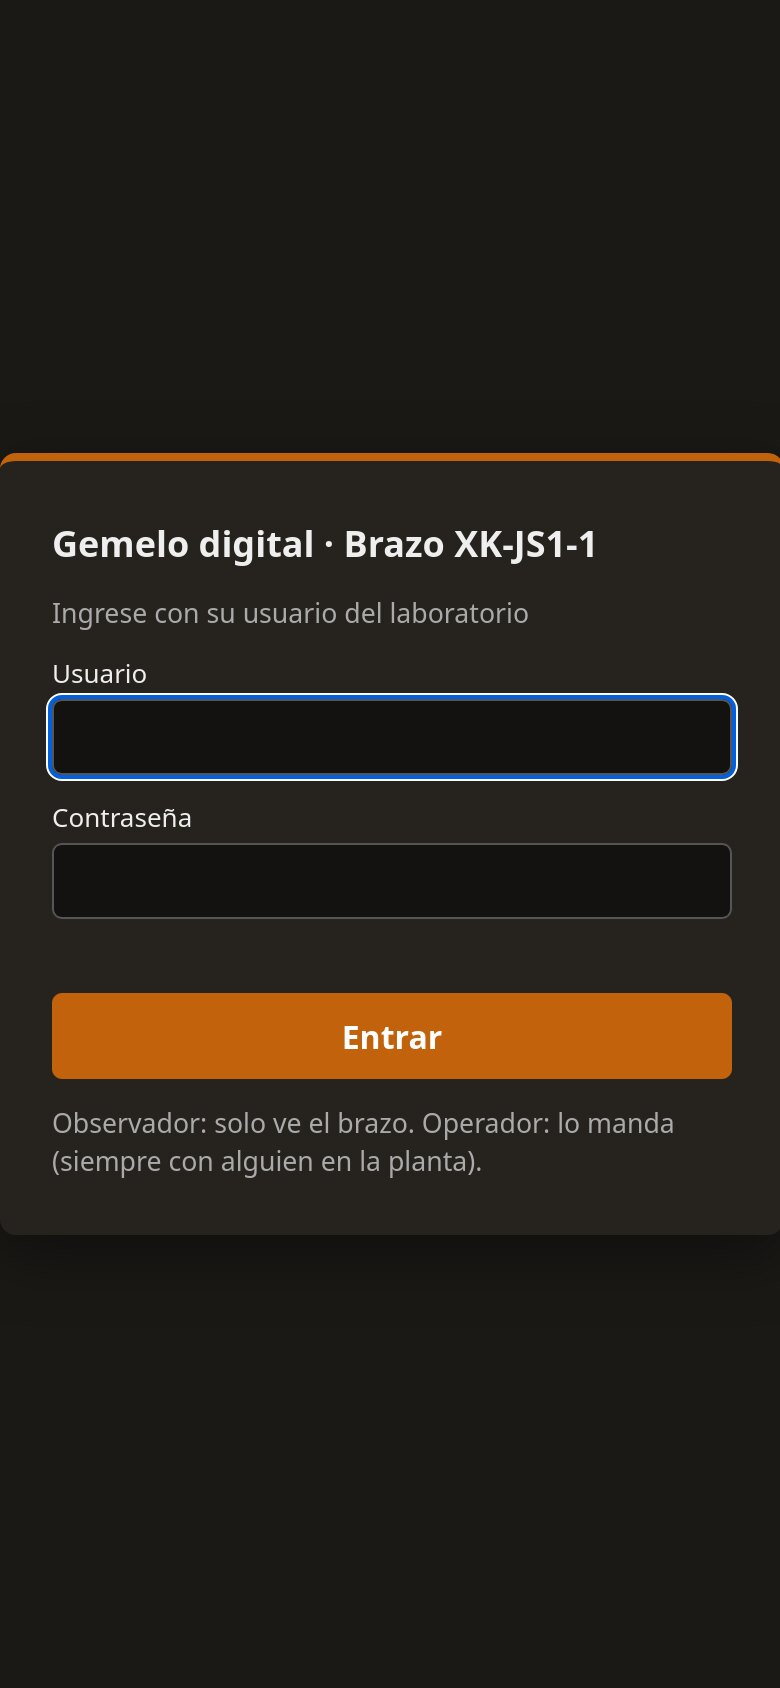
\includegraphics[width=\linewidth]{img/remoto_login.jpg}\\[2pt]{\small (a) ingreso}
\end{minipage}\hfill
\begin{minipage}[t]{0.31\linewidth}\centering
\captura{\linewidth}{img/remoto_observador.jpg}{
  \node[marca] at (0.80,0.955) {1};
  \node[marca] at (0.50,0.905) {2};
  \node[marca] at (0.07,0.03) {3};
}\\[2pt]{\small (b) observador}
\end{minipage}\hfill
\begin{minipage}[t]{0.31\linewidth}\centering
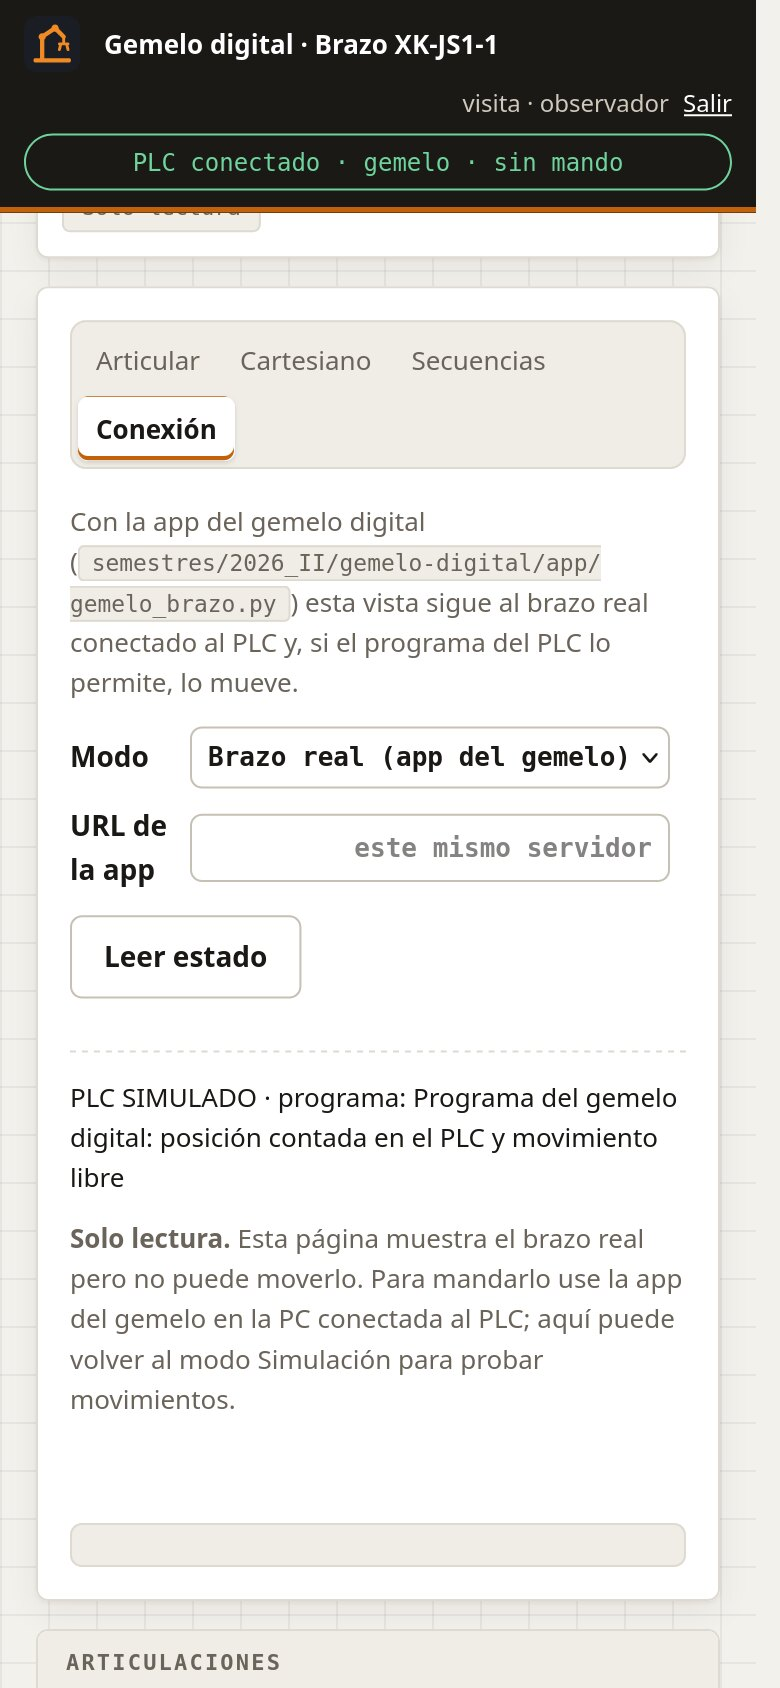
\includegraphics[width=\linewidth]{img/remoto_observador_conexion.jpg}\\[2pt]{\small (c) observador, Conexión}
\end{minipage}
\caption{Acceso remoto desde un celular como \textbf{observador}.}
\end{figure}
\begin{enumerate}[label=\num{\arabic*}, leftmargin=9mm]
\item Usuario y rol, y \emph{Salir} para cerrar la sesión. Desde la red no aparece el botón «Menú»: el modo solo se cambia en la PC del laboratorio.
\item Estado: PLC conectado, programa y quién tiene el mando.
\item \emph{Solo lectura}: los controles aparecen bloqueados. Si igual intenta mandar, la app lo rechaza y lo anota en el registro.
\end{enumerate}

\begin{figure}[H]
\centering
\begin{minipage}[t]{0.31\linewidth}\centering
\captura{\linewidth}{img/remoto_operador_conexion_antes.jpg}{\node[marca] at (0.05,0.34) {1};}\\[2pt]{\small (a) operador, sin mando}
\end{minipage}\hfill
\begin{minipage}[t]{0.31\linewidth}\centering
\captura{\linewidth}{img/remoto_operador_conexion.jpg}{\node[marca] at (0.06,0.905) {2}; \node[marca] at (0.05,0.40) {3};}\\[2pt]{\small (b) mando tomado}
\end{minipage}\hfill
\begin{minipage}[t]{0.31\linewidth}\centering
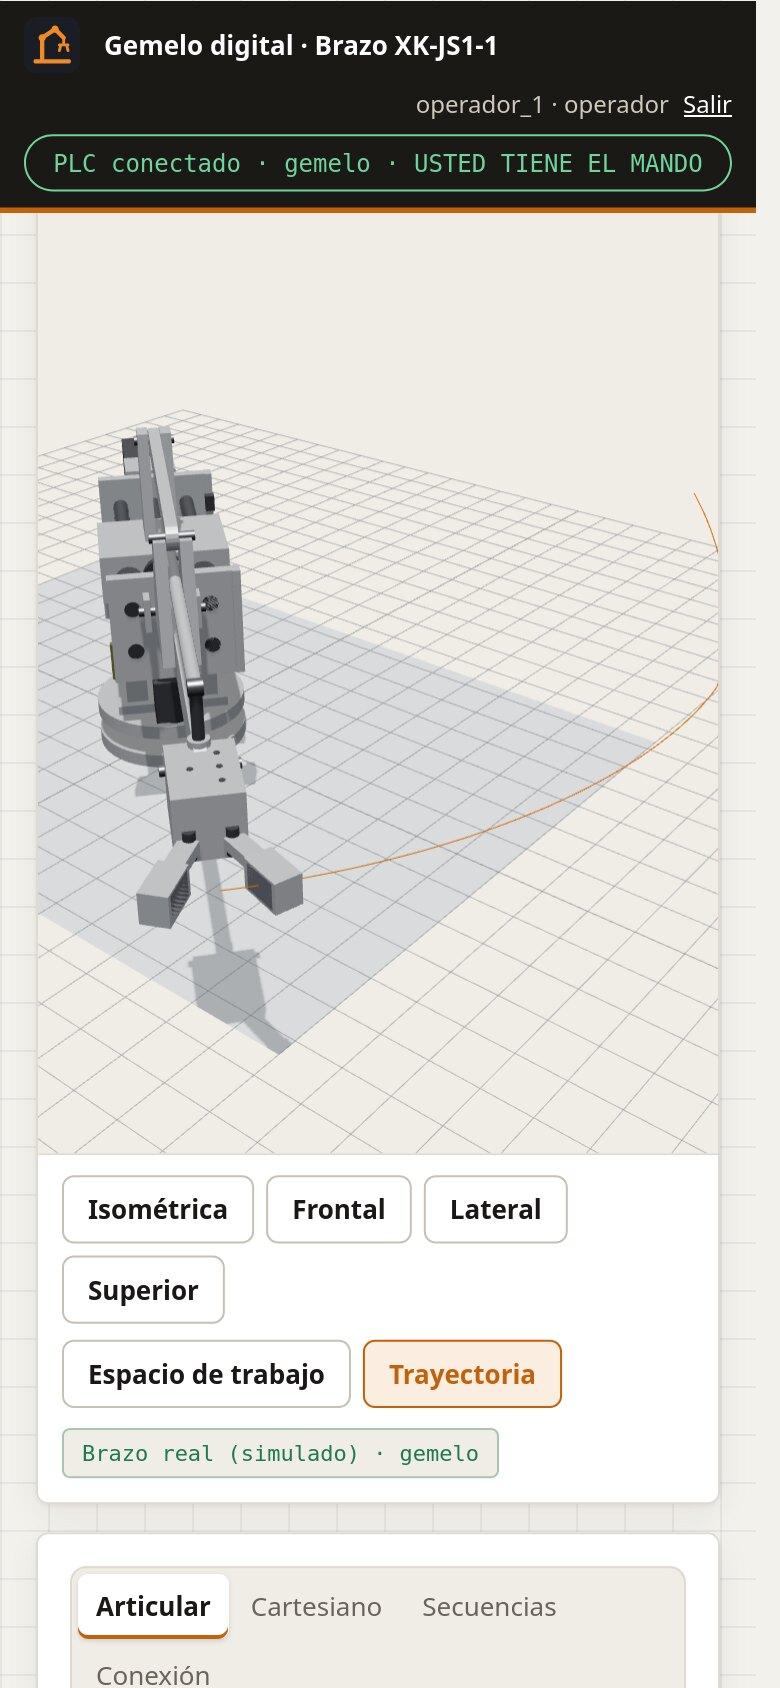
\includegraphics[width=\linewidth]{img/remoto_operador_mueve.jpg}\\[2pt]{\small (c) el brazo se movió}
\end{minipage}
\caption{Acceso remoto como \textbf{operador}.}
\end{figure}
\begin{enumerate}[label=\num{\arabic*}, leftmargin=9mm]
\item Al ingresar, el operador no tiene el mando: la casilla \emph{Habilitar el mando} está vacía.
\item Al marcarla y confirmar, el estado pasa a \emph{USTED TIENE EL MANDO}.
\item Desde ahí usa las pestañas igual que en la PC del laboratorio (sección \ref{sec:gemelo}).
\end{enumerate}

\nota{\textbf{La app debe estar abierta en la PC del laboratorio} mientras se use el brazo desde los celulares: es la única que habla con el PLC. Si se cierra, los celulares ven \emph{Sin conexión} y el PLC detiene cualquier movimiento en curso. El acceso llega solo a la red local; para usarlo desde internet haría falta una VPN.}

\subsection{Comprobar qué hace cada usuario}
La consola de la app y el archivo \codigo{registro\_gemelo.log} muestran los ingresos y las órdenes:
\begin{lstlisting}
00:59:50 modo: Operación por red local
00:59:55 ingreso de visita (observador) desde 192.168.1.20
01:00:12 RECHAZADO /api/orden/mover de visita (observador): solo puede ver
01:00:20 ingreso de operador_1 (operador) desde 192.168.1.9
01:00:25 mando desde la PC HABILITADO (operador_1)
01:00:31 orden homing  (operador_1)
\end{lstlisting}

% =====================================================================
\section{La página pública}
La página publicada en internet (\url{https://brazo-4gdl-gemelo-digital.pages.dev}) sirve para estudiar y simular el brazo. Abierta en la propia PC del laboratorio, con la app en marcha, puede además \emph{ver} el brazo real (pestaña \emph{Conexión}, modo \emph{Brazo real}, URL \codigo{http://localhost:8050}), pero nunca mandarlo.

% =====================================================================
\section{Solución de problemas comunes}
\begin{center}\small
\begin{longtable}{>{\raggedright}p{5.4cm} >{\raggedright\arraybackslash}p{10.4cm}}
\toprule
\textbf{Síntoma} & \textbf{Qué hacer}\\
\midrule
\endhead
Estado: \emph{no hay ningún puerto serie} & El cable no está enchufado o le falta el driver.\\
Estado: \emph{no responde ningún PLC} & PLC apagado o en STOP, cable fuera del puerto 0, o Micro/WIN tiene el puerto abierto.\\
\emph{para la operación por red cree antes al menos un usuario} & Cree un usuario en el panel \emph{Usuarios} del menú.\\
\emph{no se pudo abrir el acceso por red} & Otro programa usa el puerto 8443 (por ejemplo, otra copia de la app abierta). Ciérrela.\\
El celular no abre la página & Use \codigo{https://} y \codigo{:8443}; mismo Wi-Fi; revise el cortafuegos (sección de instalación). Redes de invitados pueden aislar a los equipos.\\
\emph{La conexión no es privada} & Normal la primera vez: \emph{Avanzado $\rightarrow$ Continuar}.\\
\emph{Usuario o contraseña incorrectos} & El nombre distingue mayúsculas. Cambie la contraseña desde el menú.\\
\emph{su usuario es observador} & Ese usuario solo puede ver: cambie su rol a operador en el menú.\\
\emph{Mando en uso por \dots} & Otro operador tiene el mando: puede dar paro, pero no mover hasta que lo suelte.\\
\emph{el mando desde la PC está deshabilitado} & Marque \emph{Habilitar el mando} en la pestaña \emph{Conexión}.\\
\emph{Selector en manual} & Gire el selector del panel a automático.\\
\emph{falta hacer homing} & Use \emph{Homing}.\\
\emph{Inalcanzable} en \emph{Cartesiano} & Use \emph{Usar ese punto} o cambie los valores de a poco.\\
\emph{watchdog} & La página o la app dejaron de responder durante un movimiento: vuelva a hacer homing.\\
El modelo no coincide con el brazo & Haga homing.\\
\bottomrule
\end{longtable}
\end{center}


% =====================================================================
\section{Convertidor USB--RS485 en lugar del cable USB-PPI}\label{sec:rs485}
El puerto del S7-200 es RS-485, así que un convertidor USB--RS485 \textbf{con cambio de dirección automático} debería servir (por comprobar en la planta): A(+) al pin 3 del DB9, B($-$) al pin 8 y GND al pin 5. Si el PLC no responde, invierta A y B. Windows lo mostrará como otro puerto COM y la app lo buscará igual. Conviene uno con aislamiento galvánico. Pruébelo primero con \archivo{Probar conexion PLC.bat}.

% =====================================================================
\section{Problemas propios de Windows}
\begin{center}\small
\begin{longtable}{>{\raggedright}p{5.4cm} >{\raggedright\arraybackslash}p{10.4cm}}
\toprule
\textbf{Síntoma} & \textbf{Qué hacer}\\
\midrule
\endhead
\emph{No se encontró Python} & Instale Python (paso 2) marcando \emph{Add python.exe to PATH}.\\
Se abre la Microsoft Store al escribir \codigo{python} & Es un acceso de Windows, no Python. Instale Python desde python.org; el \codigo{.bat} usa \codigo{py}.\\
La consola se cierra enseguida & Ábrala desde un \emph{Símbolo del sistema} para leer el error: \codigo{cd C:\textbackslash GemeloBrazo} y luego \codigo{py gemelo\_brazo.py}.\\
\emph{Acceso denegado} al abrir el COM & Otro programa usa el puerto (Micro/WIN, otra copia de la app). Ciérrelo.\\
La ventana del gemelo no aparece & Agregue \codigo{-{}-navegador} en el \codigo{.bat} o instale Edge o Chrome.\\
El celular no abre la página & Regla del firewall, red como \emph{Privada} (paso 4), \codigo{https://} y \codigo{:8443}.\\
\emph{Windows protegió su PC} & \emph{Más información $\rightarrow$ Ejecutar de todas formas}, o desbloquee el \codigo{.zip} (paso 1).\\
Letras raras en la consola & Solo afecta a tildes en los mensajes; no cambia el funcionamiento.\\
\bottomrule
\end{longtable}
\end{center}

\section{Desinstalar}
Borre la carpeta. Python se desinstala desde \emph{Configuración $\rightarrow$ Aplicaciones}. Si se creó la regla del firewall: \codigo{netsh advfirewall firewall delete rule name="Gemelo brazo"}.

\end{document}
